
% Eigener Beitrag: Beschreibung, Begründung, Aufzeigung, Methode, Fazit

\chapter{Anforderungen und Analyse}
\label{sec:analyse}

\section{Anaylse der travelwindow AG API}
Die \Gls{glos:api} der travelwindow AG ist mit \Gls{glos:hal} aufgebaut. Sprich es gibt einen Einstiegspunkt, welcher unter "`/"' erreichbar ist. Danach navigiert man sich über Links durch die Schnittstelle durch. Dies macht die API frei erkundbar, jedoch die Umsetzung mittels BPMN komplexer.

Nachfolgend werden die benötigten Anfragen an die API aufgeführt, welche für die Suche eines Hotel und Flug Angebotes benötigt werden (siehe \cref{sec:Recherche:rahmenbedingungen:prozesse} \nameref{sec:Recherche:rahmenbedingungen:prozesse}). Die aufgeführten Antworten sind für eine bessere Übersichtlichkeit verkürzt.


\begin{lstlisting}[language=json,firstnumber=1]
{
	test: "haha",
	"blubb": 1
}
\end{lstlisting}

\section{Bonita}
Also BPMN Programm wurde Bonita festgelegt (siehe \cref{sec:Recherche:programme:analyse} \nameref{sec:Recherche:programme:analyse}). In diesem Abschnitt wird eine Einführung in das Tool gegeben. 

Bonita besteht aus einem Programm, welches in Java geschrieben ist, sowie aus einem Webseite, welcher standardmässig auf einem mitgelieferten Tomcat Webserver\footcite{Tomcat_2016-06-12} läuft.
Nachfolgend wird das Interface des Programmes und die verwendeten Funktionen der Software beschrieben.

\subsection{Interface}
Wenn man ein neues Projekt erstellt, sieht das Programm folgendermassen aus:
\begin{figure}[H]
	\centering
	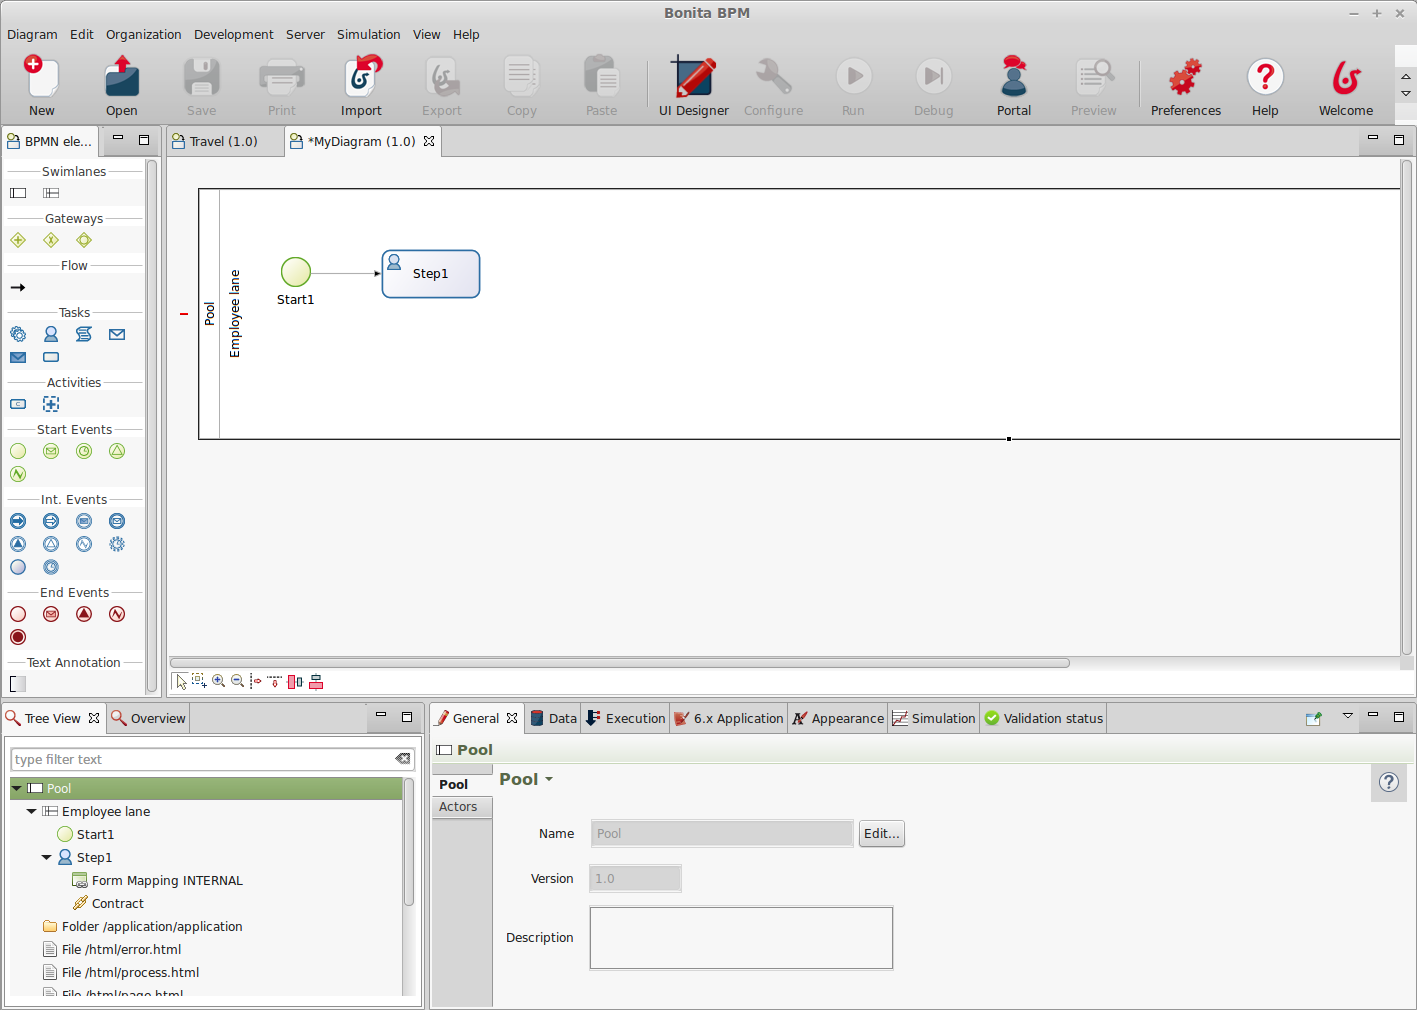
\includegraphics[width=1\textwidth]{images/bonita.png}
	\caption{Bonita Interface}
	\label{fig:analyse:bonita:interface}
\end{figure}
Zuoberst ist die Toolbar. Darunter auf der linken Seite sind die BPMN Elemente (siehe \cref{sec:Recherche:bpmn:notation} \nameref{sec:Recherche:bpmn:notation}) wie z.B. die Swimlanes, Gateways und Events. Daneben kann der Prozess definiert werden in der Process View. Bei einem neuen Projekt hat es einen Start Event (mit dem Namen "`Start1"') und ein Task "`Step1"'. Bei dem Task hat es links oben ein Benutzer Icon. Dieses sagt aus, dass es sich um einen Human Task handelt, bei welchem eine Benutzerinteraktion benötigt wird.

Zuunterst links ist eine Übersicht über alle Elemente im Projekt (Tree View) und daneben können die BPMN Elemente im Projekt konfiguriert werden (Configuration View).

Bonita ist mit Java implementiert. Auch die Erweiterungen (siehe \cref{sec:analyse:bonita:connectors} \nameref{sec:analyse:bonita:connectors}) werden in dieser Sprache entwickelt. Für das Verständnis wird vorausgesetzt, dass man grundlegendes Wissen für Java Begriffe besitzt (z.B. Namespace, Class, Implementation, Interface, etc.).

\subsection{Business Data Model}
\gls{bdm} werden für die Modellierung der Daten benötigt. Connectoren können später diese Daten entgegen nehmen oder zurückgeben. Intern handelt es sich dabei um Java Classes.

Ein \gls{bdm} hat einen Namen und Felder. Felder haben wiederum einen Namen und einen Java Datentypen (string, int oder ein weiteres \gls{bdm}). Ein Feld kann zusätzlich noch die zwei Attribute Multiple oder Mandatory haben. Ist Multiple gesetzt, so handelt es sich bei dem Feld um eine Liste, und Mandatory macht es zwingend, dass bei der Erstellung ein Wert zugewiesen wird.

\begin{figure}[H]
	\centering
	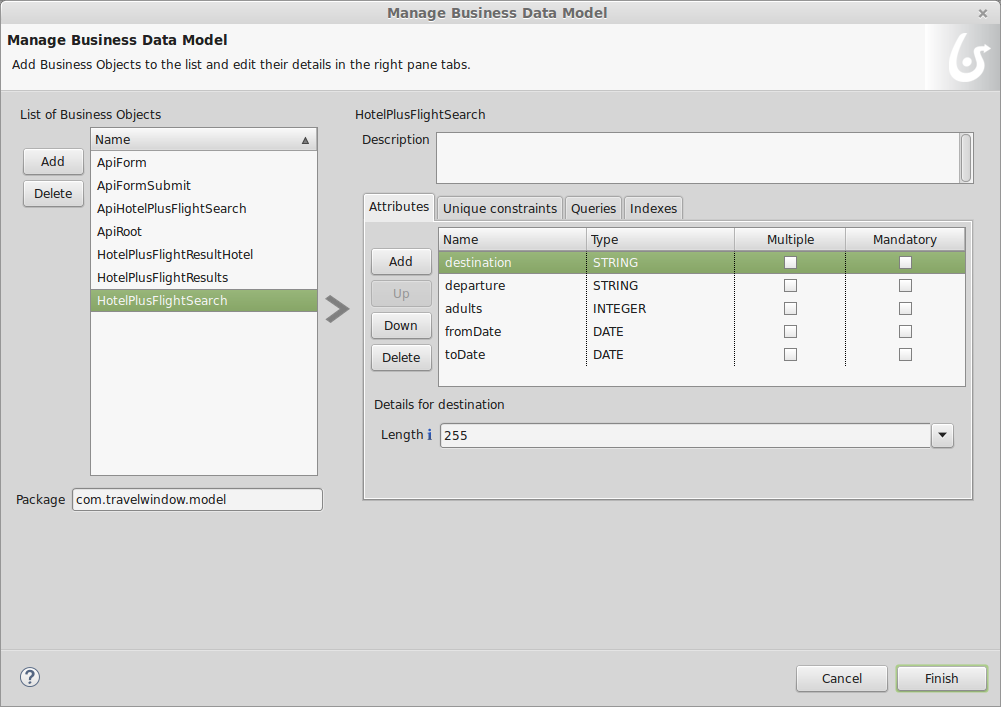
\includegraphics[width=0.8\textwidth]{images/bonita-bpm.png}
	\caption{Bonita BPM}
	\label{fig:analyse:bonita:bpm}
\end{figure}

\subsubsection{Pool Variables}
Ist in der Process View ein Pool angewählt, so kann in der Configuration View unter "`Data -> Pool Variables"' neue Pool Variablen definiert werden. Diese sind für alle Tasks in diesem Pool und Swimplanes sichtbar und können von den Connectors verwendet werden. Dabei handelt es sich um Instanzen von \glspl{bdm}. Eine Pool Variable besteht aus einem Namen, einem \gls{bdm} und einem Initialisierungs-Skript, um die Mandatory Fields abzufüllen.
\begin{figure}[H]
	\centering
	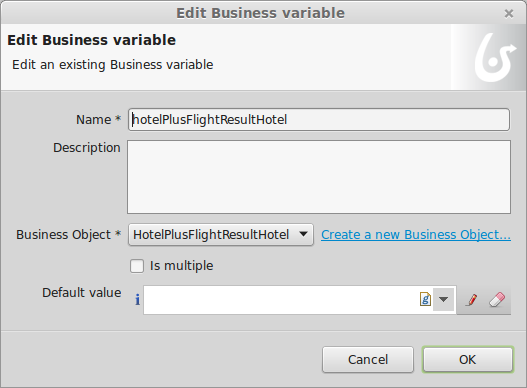
\includegraphics[width=0.8\textwidth]{images/bonita-poolvariables.png}
	\caption{Bonita Pool Variables}
	\label{fig:analyse:bonita:bpm:poolvariables}
\end{figure}

\subsection{Connectors}
\label{sec:analyse:bonita:connectors}
Connectors werden in Bonita dazu verwendet, um eine Aktion durchzuführen. 

Bonita wird mit folgenden Connectors ausgeliefert:
\begin{itemize}
\item CMS
\item CRM
\item Calendar
\item Database
\item ERP
\item LDAP
\item Messaging
\item Reporting
\item SOAP Web Services
\item Script
\item Social
\item Talend
\end{itemize}

Connectors können einem Task angehängt werden. Klickt man einen Task in der Process View an, kann man in der Configuration View unter Execution Connectors hinzufügen.
\begin{figure}[H]
	\centering
	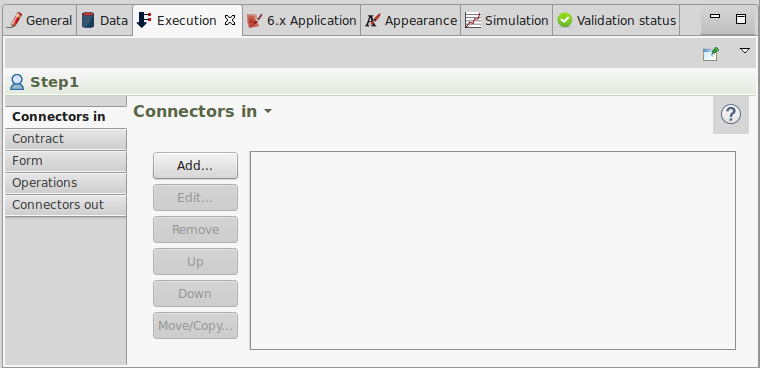
\includegraphics[width=1\textwidth]{images/bonita-connectors.png}
	\caption{Bonita Connectors}
	\label{fig:analyse:bonita:connectors}
\end{figure}
Es gibt in und out Connectors. Diese werden entweder vor dem Task, oder nach dem Task ausgeführt. Bei einem Human Task kann so definiert werden, ob der Connector vor der Benutzerinteraktion ausgeführt wird oder danach.

Ein Connector besteht aus einer Definition und einer Implementation, welche nachfolgend beschrieben sind. In der Definition ist spezifiziert, was die Eingaben und Ausgaben sind. Wird ein Connector einem Task angehängt, so müssen die Eingaben definiert sowie ein Mapping der Ausgabeparameter gemacht werden.

\subsubsection{Definition}
Die Definition eines Connectors besteht aus Beschreibungsdaten (Name, Namespace, Kategorie, etc.), Input-Parameter, Wizard Pages und Output-Parameter. Als Input- und Output-Parameter können Java Classes oder \glspl{bdm} definiert werden. Wizard Pages werden dazu benötigt, dass wenn ein Connector einem Task hinzugefügt wird die entsprechenden Input-Parameter definiert werden können.

\subsubsection{Implementation}
Um eine Implementation eines Connectors anzulegen, muss zuerst eine Definition gewählt und Beschreibungsdaten angeben werden.
\begin{figure}[H]
	\centering
	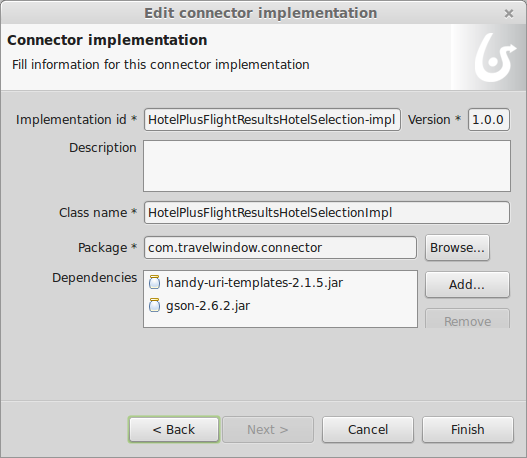
\includegraphics[width=1\textwidth]{images/bonita-connectors-implementation.png}
	\caption{Bonita Connector Implementation}
	\label{fig:analyse:bonita:connectors:implementation}
\end{figure}
Die Implementation id kann frei gewählt werden, muss im Projekt jedoch eindeutig sein. Der Class name ist der Name der Java Klasse die erstellt wird. Dependencies sind JAR Files welche von innerhalb der Java Klasse benötigt werden.

Bestätigt man den obigen Dialog, so wird eine Java Klasse und abstrakte Klasse erzeugt. Nach dem obigen Beispiel werden die beiden Classes HotelPlusFlightResultsHotelSelectionImpl und AbstractHotelPlusFlightResultsHotelSelectionImpl erstellt. Das Hauptmethode der ersteren ist die Methode executeBusinessLogic. In der Definition dieses Connectors wurde definiert, dass ein \gls{bdm} HotelPlusFlightResultHotel zurückgegeben wird, welches den namen "`selection"' hat. Deshalb muss die Methode executeBusinessLogic die Methode "`setSelection"' aufrufen und dieser eine Classe vom Typen HotelPlusFlightResultHotel übergeben, um der Definition zu genügen. 
Die Methode setSelection ist dabei in der AbstractHotelPlusFlightResultsHotelSelectionImpl definiert.

Die Funktionalität eines Connectors kann somit frei implementiert werden. Zwingend ist nur das die Methode setSelection aufgerufen wird, sonst die die Ausführung des Connectors fehlerhaft.

\subsection{Forms, Contracts und Operations}
\label{sec:analyse:bonita:forms}
Bei einem Human Task muss ein Form angehängt werden, um dem Benutzer eine Interaktion in dem Prozess zu ermöglichen.
In einem Task kann direkt ein neues Formular erstellt werden. Es empfiehlt sich jedoch, zuerst den Contract zu definieren, da die dort angegeben Informationen automatisch bei der Erstellung des Forms und den Operations mitberücksichtigt werden. Weitere Informationen dazu werden den folgenden beiden Abschnitten gegeben.

\subsubsection{Contract}
\label{sec:analyse:bonita:forms:contract}
Ein Contract definiert die Daten, die vom Formular erwartet werden. Sie sind dafür verantwortlich, welche Informationen aus dem Process an das Form übergeben werden. Die dort definierten Werte können Java Klassen oder \glspl{bdm} sein. Beim Task für die Auswahl eines Hotels in der Hotel und Flug suche, könnte dies die Liste der Hotelresultate sein. Dazu wird im Contract eine Liste von Hotels angegeben.
\begin{figure}[H]
	\centering
	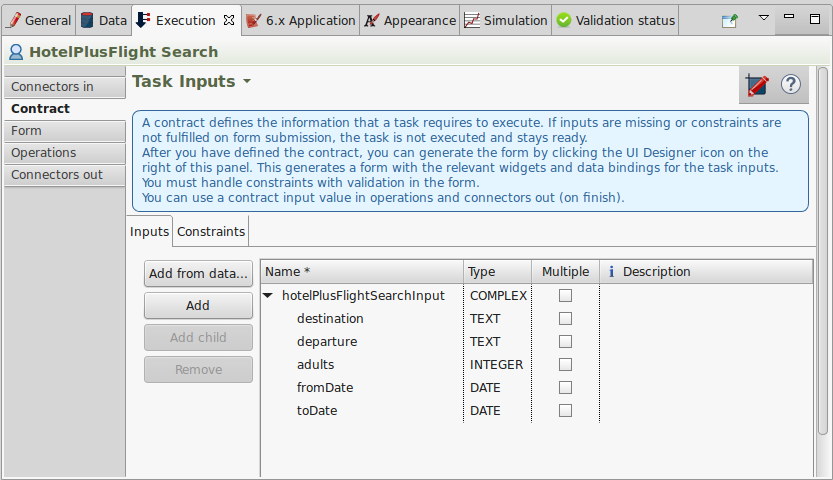
\includegraphics[width=1\textwidth]{images/bonita-contract.png}
	\caption{Bonita Form Contract}
	\label{fig:analyse:bonita:forms:contract}
\end{figure}

\subsubsection{Operations}
\label{sec:analyse:bonita:forms:operations}
Operations werden nach der Ausführung des Formulars ausgeführt. Sie definieren, wie die Informationen aus dem Formular zurück in den Prozess fliessen.

\begin{figure}[H]
	\centering
	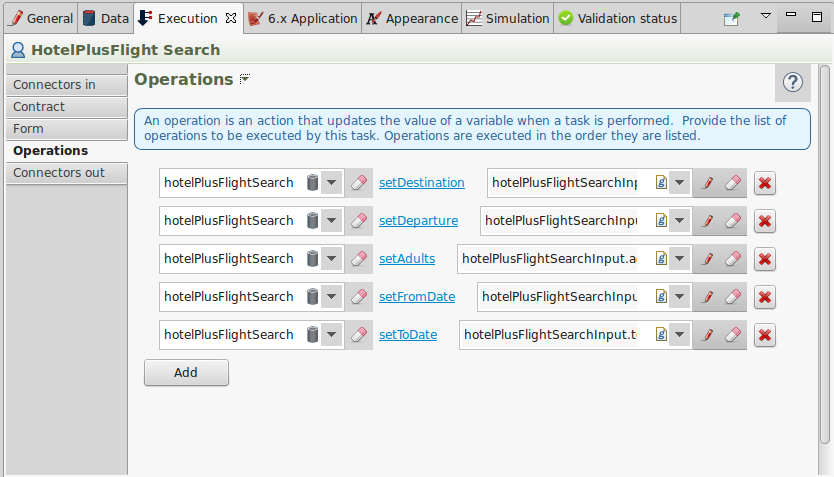
\includegraphics[width=1\textwidth]{images/bonita-operations.png}
	\caption{Bonita Form Operations}
	\label{fig:analyse:bonita:forms:operations}
\end{figure}
Im obigen Beispiel wird definiert, dass auf der Pool Variable hotelPlusFlightSearch die Java Methode setDestination aufgerufen wird. Der Methode wird der Wert hotelPlusFlightSearchInput.destination übergeben. Bei hotelPlusFlightSearchInput handelt es sich um eine Variable, welche auf dem Formular definiert wurde (siehe \nameref{sec:analyse:bonita:forms:forms}).

\subsubsection{Forms}
\label{sec:analyse:bonita:forms:forms}
Ein Form ermöglicht die Interaktion eines Benutzers. Die Daten die an das Form übergeben werden und wie die bearbeiteten Daten zurück in den Process fliessen, ist in dem Contract und den Operations definiert (siehe \nameref{sec:analyse:bonita:forms:contract} und  \nameref{sec:analyse:bonita:forms:operations}). Es ist zu empfehlen, dass zuerst diese beiden Informationen definiert werden, da sie bei der Erstellung des Forms direkt weiterverwendet werden. Definiert man bei dem Contract dass eine Liste von Hotels übergeben wird, so wird bei der Erstellung des Formulars automatisch eine Liste generiert welche diese Daten anzeigt. 

Um ein Formular aus den Daten des Contracts und der Operations zu erstellen, muss dieses in der Configuration View erstellt werden.
\begin{figure}[H]
	\centering
	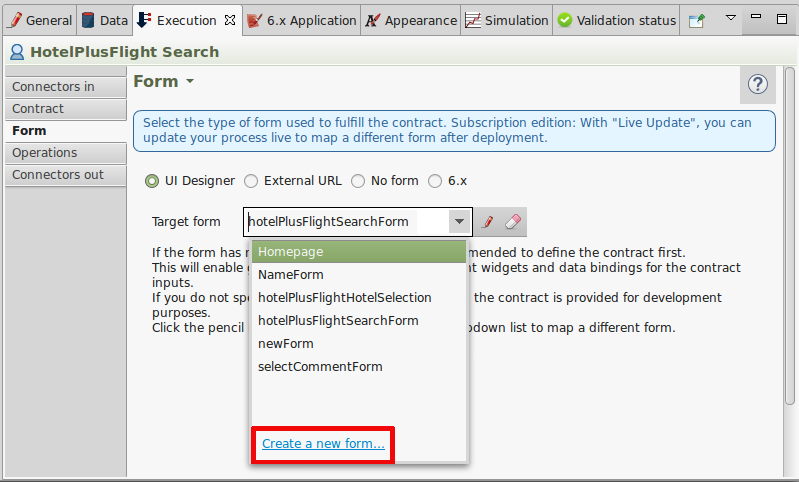
\includegraphics[width=1\textwidth]{images/bonita-forms-create.png}
	\caption{Bonita Form erstellung aus Contract und Operations}
	\label{fig:analyse:bonita:forms:forms:creation}
\end{figure}

Danach öffnet sich der UI Designer. Dies ist ein Webinterface, welches auf dem mitgelieferten Tomcat Webserver läuft. Dort kann das Formular angepasst werden.
Die Funktionalität des UI Designers ist gross. Einen guten Überblick bietet ein Video Tutorial, welches von Bonitasoft bereit gestellt wird und auf folgender URL eingesehen werden kann \url{http://www.bonitasoft.com/resources/videos/getting-started-tutorial}. Ab 35:55 wird der UI Designer vorgestellt.